\section{Loss function}

Consider an independent and identically distributed sample drawn from a Gaussian distribution with a known variance, $\sigma^2$.
The goal is to estimate the parameter $\mu$ using Maximum Likelihood Estimation (MLE), which selects parameters that maximize the probability of the observed data.

Let $\boldsymbol{\theta}=\begin{pmatrix} \theta_1 & \theta_2 & \dots & \theta_p \end{pmatrix}^T$ represent the vector of parameters. 
The task is to find the MLE of $\boldsymbol{\theta}$.
Here is the step-by-step approach:
\begin{enumerate}
    \item \textit{Construct the likelihood function}: the likelihood function $L(\mu)$ is the probability of the data given $\mu$, assuming a Gaussian distribution. 
        The joint likelihood of the data $x_1,x_2,\dots,x_N$ is: 
        \[L(\mu)=\Pr(x_1,x_2,\dots,x_N|\mu,\sigma^2)=\prod_{n=1}^N\Pr(x_n|\mu,\sigma^2)=\prod_{n=1}^N\dfrac{1}{\sqrt{2\pi}}e^{-\dfrac{(x_n-\mu)^2}{2\sigma^2}}\]
    \item \textit{Log-likelihood function}: since the likelihood is a product, it is convenient to take the logarithm to transform it into a sum, yielding the log-likelihood: 
        \[l(\mu)=\log\left(\prod_{n=1}^N\dfrac{1}{\sqrt{2\pi}}e^{-\dfrac{(x_n-\mu)^2}{2\sigma^2}}\right)=\sum_{n=1}^N\log\dfrac{1}{\sqrt{2\pi}}e^{-\dfrac{(x_n-\mu)^2}{2\sigma^2}}\]    
        Simplifying:
        \[l(\mu)=N\log\dfrac{1}{\sqrt{2\pi}}-\dfrac{1}{2\sigma^2}\sum_n^N(x_n-\mu)^2\]
    \item \textit{Compute the gradient of the log-likelihood}: to find the MLE for $\mu$, we need to maximize the log-likelihood by taking its derivative with respect to $\mu$ and setting it to zero:
        \[\dfrac{\partial l(\mu)}{\partial \mu}= \dfrac{\partial}{\partial \mu} \left( N \log \dfrac{1}{\sqrt{2 \pi} \sigma} - \dfrac{1}{2 \sigma^2} \sum_n^N (x_n - \mu)^2 \right)\]
        Focusing on the second term, the derivative is:
        \[\dfrac{\partial l(\mu)}{\partial \mu}=-\dfrac{1}{2 \sigma^2} \dfrac{\partial}{\partial \mu} \sum_n^N (x_n - \mu)^2 = \dfrac{1}{2 \sigma^2} \sum_n^N 2(x_n - \mu)\]
    \item \textit{Solve the equation for MLE}: setting the derivative equal to zero to maximize the likelihood:
        \[\dfrac{1}{2 \sigma^2} \sum_n^N 2(x_n - \mu)=0\]  
        This simplifies to:
        \[\sum_n^N x_n=\sum_n^N \mu\]   
        Hence, the MLE for $\mu$ is:
        \[\mu^{\text{MLE}}=\dfrac{1}{N}\sum_n^Nx_n\]
        This is the sample mean, which is the optimal estimate for $\mu$ under the MLE framework.
\end{enumerate}
To maximize or minimize the log-likelihood, we can apply several techniques:
\begin{itemize}
    \item \textit{Analytical methods}: directly solve the equations for the MLE, as done above.
    \item \textit{Optimization techniques}: use methods such as Lagrange multipliers for constrained optimization problems.
    \item \textit{Numerical methods}: apply iterative approaches like gradient descent when closed-form solutions are intractable.
\end{itemize}
In our case, we derived the MLE for $\mu$ analytically as the sample mean, but for more complex models, numerical optimization techniques may be necessary.
\begin{example}
    Consider the following Feed Forward Nwural Network. 
    \begin{figure}[H]
        \centering
        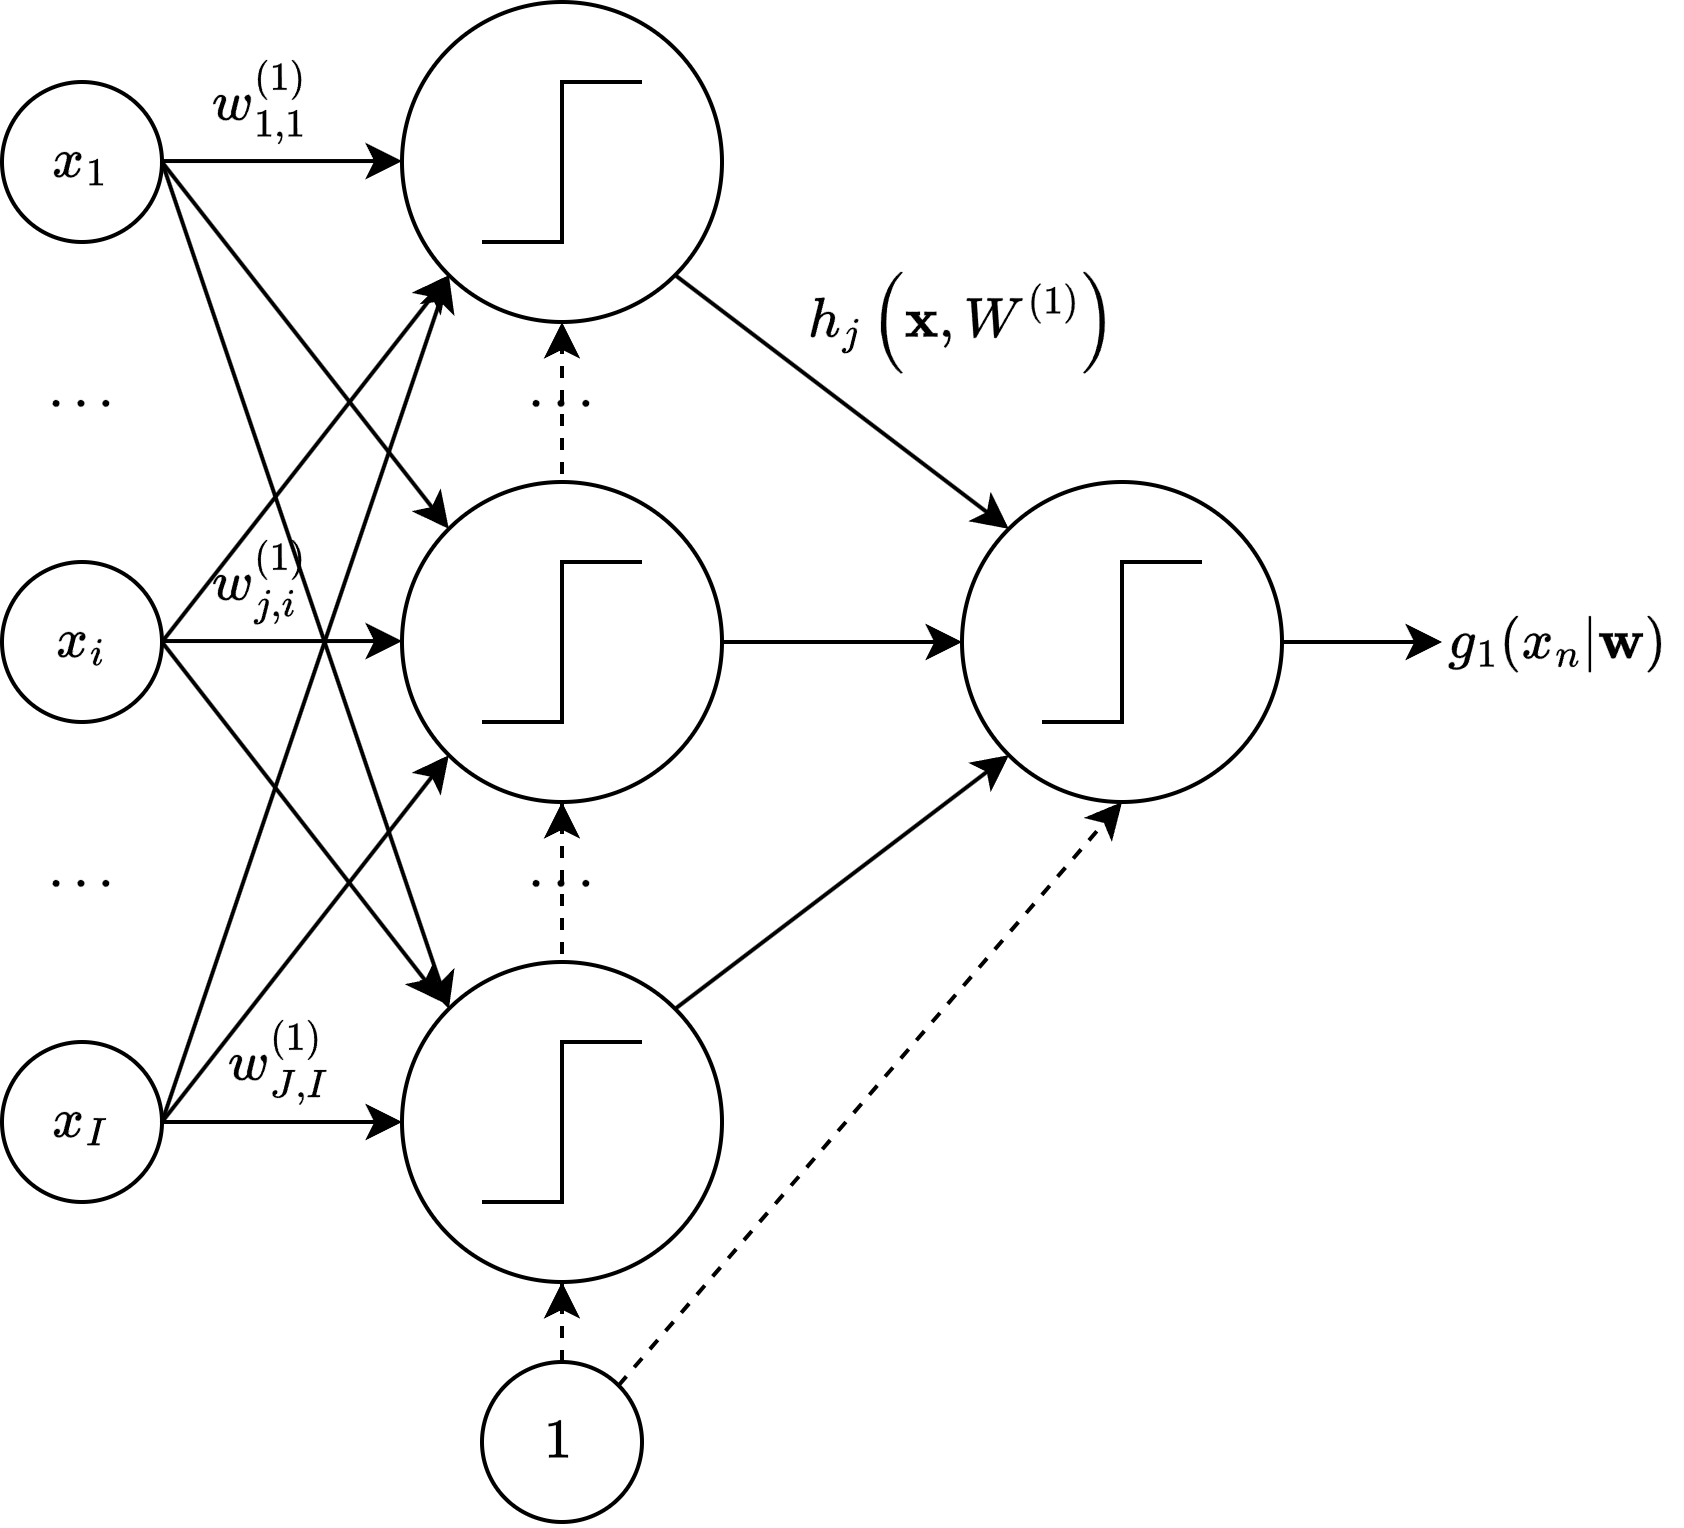
\includegraphics[width=0.7\linewidth]{images/ffnn1.png}
    \end{figure}
    The output of the network is defined as:
    \[g_1(x_n|\mathbf{w})=g_1\left(\sum_{j=0}^Jw_{1,j}^{(2)}h_j\left(\sum_{i=0}^Iw_{j,i}^{(1)}x_{i,n}\right)\right)\]
    Here, $h_j$ represents the activation function of the hidden neurons, and $w_{i,j}^{(1)}$ and $w_{i,j}^{(2)}$ are the weights of the first and second layers, respectively.
    The goal is to approximate a target function $t$ having $N$ observations: 
    \[t_n=g(x_n|\mathbf{w})+\epsilon_n \qquad \epsilon_n\sim N(0,\sigma^2)\rightarrow t_n\sim N(g(x_n|\mathbf{w}),\sigma^2)\]

    To estimate the weights $\mathbf{w}$ in a model $g(x_n|\mathbf{w})$ using Maximum Likelihood Estimation (MLE), follow these steps:
    \begin{enumerate}
        \item \textit{Write the likelihood function $L(\mathbf{w}) = P(\text{data}|\mathbf{w})$ for the data}: assume that the observed values $t_n$ are drawn from a Gaussian distribution with known variance $\sigma^2$, and that the model $g(x_n|\mathbf{w})$ provides the mean of the distribution. The probability of each observation is given by:
            \[\Pr(t_n|g(x_n|\mathbf{w}), \sigma^2) = \dfrac{1}{\sqrt{2\pi\sigma^2}} e^{-\dfrac{(t_n - g(x_n|\mathbf{w}))^2}{2\sigma^2}}\]
            The likelihood function for the entire dataset is the product of these probabilities:
            \[L(\mathbf{w}) = \Pr(t_1, t_2, \dots, t_N|g(x|\mathbf{w}), \sigma^2) = \prod_{n=1}^N \Pr(t_n|g(x_n|\mathbf{w}), \sigma^2)\]
            Substituting the expression for each $\Pr(t_n)$, we get:
            \[L(\mathbf{w}) = \prod_{n=1}^N \dfrac{1}{\sqrt{2\pi\sigma^2}} e^{-\dfrac{(t_n - g(x_n|\mathbf{w}))^2}{2\sigma^2}}\]
        \item \textit{Write the log-likelihood function $l(\mathbf{w}) = \log P(\text{data}|\mathbf{w})$} :taking the logarithm of the likelihood function simplifies the product into a sum:
            \[l(\mathbf{w}) = \log\left( \prod_{n=1}^N \dfrac{1}{\sqrt{2\pi\sigma^2}} e^{-\dfrac{(t_n - g(x_n|\mathbf{w}))^2}{2\sigma^2}} \right)\]
            This simplifies to:
            \[l(\mathbf{w}) = \sum_{n=1}^N \log \dfrac{1}{\sqrt{2\pi\sigma^2}} - \dfrac{(t_n - g(x_n|\mathbf{w}))^2}{2\sigma^2}\]
            Further simplifying:
            \[l(\mathbf{w}) = N \log \dfrac{1}{\sqrt{2\pi\sigma^2}} - \dfrac{1}{2\sigma^2} \sum_{n=1}^N (t_n - g(x_n|\mathbf{w}))^2\]
        \item \textit{Optimize the weights $\mathbf{w}$ to maximize the log-likelihood}: to find the weights $\mathbf{w}$ that maximize the log-likelihood, we solve the following optimization problem:
            \[\mathbf{w}^{\text{MLE}} = \argmax_{\mathbf{w}} l(\mathbf{w})\]
            This is equivalent to minimizing the sum of squared errors:
            \[\mathbf{w}^{\text{MLE}} = \argmin_{\mathbf{w}} \sum_{n=1}^N \left( t_n - g(x_n|\mathbf{w}) \right)^2\]
            This optimization problem is typically solved using numerical techniques like gradient descent, depending on the complexity of $g(x_n|\mathbf{w})$.
        \item \textit{Approximate the posterior probability for $t$}:f or binary classification where $t_n \in \{0, 1\}$ and $t_n \sim \text{Bernoulli}(g(x_n|\mathbf{w}))$, the likelihood for the data is given by:
            \[\Pr(t_n|g(x_n|\mathbf{w})) = g(x_n|\mathbf{w})^{t_n} \cdot (1 - g(x_n|\mathbf{w}))^{1 - t_n}\]
            The likelihood function for the entire dataset is:
            \[L(\mathbf{w}) = \prod_{n=1}^N g(x_n|\mathbf{w})^{t_n} \cdot (1 - g(x_n|\mathbf{w}))^{1 - t_n}\]
        \item \textit{Compute the log-likelihood}: taking the logarithm of the likelihood function gives:
            \[l(\mathbf{w}) = \sum_{n=1}^N \left[ t_n \log g(x_n|\mathbf{w}) + (1 - t_n) \log(1 - g(x_n|\mathbf{w})) \right]\]
            This expression is known as the cross-entropy loss:
            \[- \sum_{n=1}^N t_n \log g(x_n|\mathbf{w}) + (1 - t_n) \log(1 - g(x_n|\mathbf{w}))\]
    \end{enumerate}
\end{example}

\subsection{Loss function selection}
The choice of an appropriate loss function is crucial for defining the task and guiding the learning process. 
The loss function not only measures the error between the predicted and actual values but also influences the optimization behavior of the model. 
Designing a loss function requires careful consideration of various factors:
\begin{itemize}
    \item \textit{Leverage knowledge of the data distribution}: when selecting a loss function, it is important to incorporate any prior knowledge or assumptions regarding the underlying data distribution. 
        For example, if the data is normally distributed, a squared error loss might be appropriate, while for binary classification tasks, cross-entropy loss is typically used.
    \item \textit{Exploit task-specific and model knowledge}: a good loss function should align with the goals of the task at hand.
        For instance, in classification problems, we want to maximize the probability of correct predictions, and in regression, we aim to minimize the difference between predicted and true values. 
        Tailoring the loss function to the model and its intended use case can significantly improve performance.
    \item \textit{Creativity in loss function design}: in some cases, predefined loss functions may not fully capture the nuances of the problem, and this is where creativity can play a role. 
        Custom loss functions can be designed by combining multiple loss components or incorporating domain-specific constraints to better align with the task's objectives.
\end{itemize}
In summary, selecting the right loss function is both a science and an art—it requires a blend of theoretical insights, practical understanding of the problem domain, and sometimes, creative thinking to balance accuracy and interpretability.

\subsection{Perceptron loss function}
\paragraph*{Hyperplanes}
Consider a hyperplane $L:\mathbf{w}^T x + w_0 = 0 \in \mathbb{R}^2$. 
Any two points $x_1$ and $x_2$ lying on the hyperplane $L$ can be characterized by their relationship to this hyperplane.
The normal vector $\mathbf{w}^\ast$ to the hyperplane can be defined as follows:
\[\mathbf{w}^\ast = \dfrac{\mathbf{w}}{\|\mathbf{w}\|}\]
For any point $x_0$ on the hyperplane $L$, we can express the signed distance of any point $x$ from the hyperplane $L$ as:
\[\mathbf{w}^{\ast^T} (x - x_0)\dfrac{1}{\|\mathbf{w}\|} = \dfrac{1}{\|\mathbf{w}\|} \left( \mathbf{w}^T x + w_0 \right)\]

It can be shown that the error function minimized by the Hebbian rule is related to the distance of misclassified points from the decision boundary. 
When coding the perceptron output as $1$ or $-1$, we can represent the following conditions:
\begin{itemize}
    \item If an output that should be $1$ is misclassified, then $\mathbf{w}^T x + w_0 < 0$.
    \item Conversely, for an output that should be $-1$, we have $\mathbf{w}^T x + w_0 > 0$.
\end{itemize}
The objective then becomes to minimize the following loss function:
\[D(\mathbf{w}, w_0) = -\sum_{i \in M} t_i (\mathbf{w}^T x_i + w_0)\]
Here, $D(\mathbf{w}, w_0)$ is non-negative and proportional to the distance of the misclassified points from the decision boundary defined by $\mathbf{w}^T x + w_0 = 0$.

To minimize the error function $D(\mathbf{w}, w_0)$ using stochastic gradient descent, we take the gradients with respect to the model parameters:
\[\dfrac{\partial D(\mathbf{w}, w_0)}{\partial \mathbf{w}} = -\sum_{i \in M} t_i \cdot x_i\qquad\dfrac{\partial D(\mathbf{w}, w_0)}{\partial w_0} = -\sum_{i \in M} t_i\]
Stochastic gradient descent is applied iteratively for each misclassified point:
\[\begin{cases}
    \mathbf{w}_{k+1} = \mathbf{w}_k + \eta t_i \cdot x_i \\
    w_{0,k+1} = w_{0,k} + \eta t_i
\end{cases}\]
In this context, $\eta$ represents the learning rate. 
This iterative approach is akin to Hebbian learning and effectively implements stochastic gradient descent, allowing the perceptron to adjust its weights and bias based on the misclassified instances.

\subsection{Adaptive learning}
To effectively navigate the challenges of local minima in the optimization landscape, various techniques can be employed, one of which is momentum. 
This method helps to accelerate gradient descent in the relevant direction and dampens oscillations. 
The update rule with momentum is given by:
\[\mathbf{w}^{k+1}=\mathbf{w}^k-\eta\dfrac{\partial E(\mathbf{w})}{\partial \mathbf{w}}\Bigg|_{\mathbf{w}^k}-\alpha\dfrac{\partial E(\mathbf{w})}{\partial \mathbf{w}}\Bigg|_{\mathbf{w}^{k-1}}\]
Here, $\mathbf{w}^k$ represents the weights at iteration $k$, $\eta$ is the learning rate, and $\alpha$ is the momentum term.

\paragraph*{Nestorov accelerated gradient}
An enhancement to the momentum method is the Nesterov accelerated gradient. 
This approach first makes a momentum-based update and then adjusts the gradient based on the new position. 
The two-step update process is defined as follows:
\begin{enumerate}
    \item First, a momentum-based prediction of the next position:
        \[\mathbf{w}^{k+\frac{1}{2}}=\mathbf{w}^k-\alpha\dfrac{\partial E(\mathbf{w})}{\partial \mathbf{w}}\Bigg|_{\mathbf{w}^{k-1}}\]
    \item Then, updating the weights using the gradient evaluated at the predicted position:
        \[\mathbf{w}^{k+1}=\mathbf{w}^k-\eta\dfrac{\partial E(\mathbf{w})}{\partial \mathbf{w}}\Bigg|_{\mathbf{w}^{k+\frac{1}{2}}}\]
\end{enumerate}

\paragraph*{Layer-specific learning rates}
In deep networks, different neurons in each layer may learn at varying rates due to differences in gradient magnitudes across layers. 
Early layers are often prone to vanishing gradients, which can hinder learning. 
To address this, it is beneficial to employ separate adaptive learning rates for different layers.
Several algorithms have been proposed to achieve this:
\begin{itemize}
    \item \textit{Resilient propagation} (Rprop): introduced by Riedmiller and Braun in 1993, this algorithm adjusts the weight updates based on the sign of the gradient, ensuring that the step sizes remain appropriate.
    \item \textit{Adaptive gradient} (AdaGrad): developed by Duchi et al. in 2010, AdaGrad adapts the learning rate for each parameter based on the historical gradients, allowing for a more tailored approach.
    \item \textit{RMSprop}: a combination of Stochastic Gradient Descent and Rprop, proposed by Tieleman and Hinton in 2012. RMSprop utilizes an exponentially decaying average of squared gradients to normalize the learning rate.
    \item \textit{AdaDelta}: introduced by Zeiler et al. in 2012, this method extends AdaGrad by not accumulating past squared gradients, thus overcoming its diminishing learning rates issue.
    \item \textit{Adam} (Adaptive Moment Estimation): proposed by Kingma and Ba in 2012, Adam combines the benefits of both momentum and RMSprop, using estimates of both the first and second moments of the gradients to adaptively adjust learning rates.
\end{itemize}